\documentclass[a4paper,11pt]{article}
\usepackage[english]{babel}
\usepackage[T1]{fontenc}
\usepackage{fancyhdr}
\usepackage{graphicx}
\usepackage{caption}
\usepackage{subcaption}
\usepackage{a4wide}
\usepackage{numprint}
\usepackage{url}
\usepackage{cite}
\usepackage{multirow}
\usepackage{moreverb}
\usepackage{lastpage}
\usepackage{enumerate}
\pagestyle{fancy}

\author{Viktor Collin \\ <\url{vcollin@kth.se}> \\ 19880316-0277 \and Simon \"{O}sterman \\ <\url{simost@kth.se}> \\ 19880205-0156}
\title{\textbf{DH2323 Computer Graphics with Interaction \\ Lab 3 : Rasterisation}}

\fancyhead[L]{\textbf{DH2323 : Lab 3} }
\fancyhead[R]{Viktor Collin \& Simon \"{O}sterman : Page \thepage }
\fancyfoot{}{}

\begin{document}
\maketitle
\begin{center}
Total pages: \pageref{LastPage}
\end{center}
\thispagestyle{empty}

\clearpage
\setcounter{page}{1}
\section{Introduction}
The purpose of this lab is to learn how to build a rastreriser and use it to render an image of a 3D environment that consists of triangular shapes. The lab also includes light models and camera movement. 
\section{Assignment}
The objective of third lab is pretty much the same as in the second with the raytracing. You are supposed to create a 3D-image but instead of tracing rays you are supposed to implement a rasteriser.
\section{Method}
\subsection{First implementation}
As a first step we built our rasteriser to project the 3D-environment onto a 2D screen and then trace the vertices of each triangle and then draw the lines between the end-points \ref{fig1}. We also implemented the possibility to move the camera in the same fashion as in lab 2. 

\begin{figure}[h!]
	\centering	
	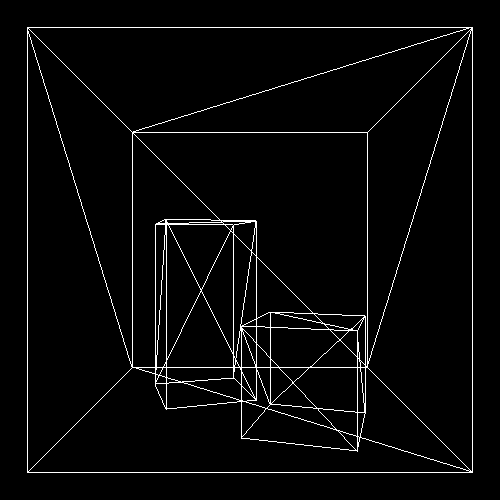
\includegraphics[width=0.45\linewidth]{screenshot1.png}
	\caption{The outlines of the polygons}
	\label{fig1}
\end{figure}
\clearpage
\subsection{Drawing Polygons}
To be able to draw the entire model, we had to go through add a lot of calculations to be able to decide which pixels was contained in each polygon. This involves first calculating the top and the bottom of the polygon as well as the leftmost and rightmost pixels.   

\begin{figure}[h!]
	\centering	
	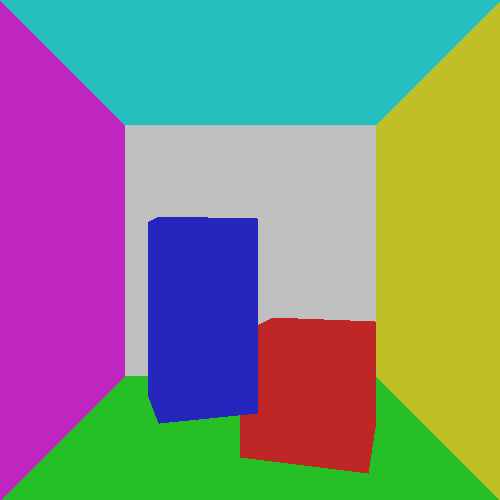
\includegraphics[width=0.45\linewidth]{screenshot15.png}
	\caption{Output of the model without using a z-buffer}
	\label{fig15}
\end{figure}

As shown in the figure \ref{fig15} the blue box is in front of the red since no z-buffer is in use.

\subsection{The z-buffer}
To be able to determine at which depth each pixel is located, a z-buffer is used. A problem with the z-buffer is that you can not use linear interpolation along the z-axis whilst using the buffer. Instead, you can linearly interpolate the z$^{-1}$ and still get a good result. Below is a print of the z-buffer:

\begin{figure}[h!]
	\centering
	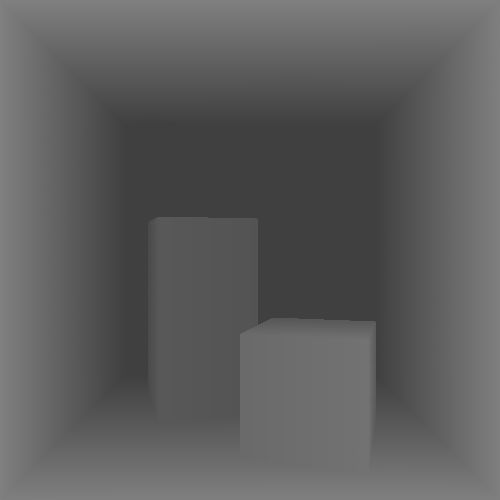
\includegraphics[width=0.40\linewidth]{screenshotz.png}
	\caption{The Z-Buffer}
	\label{figz}
\end{figure}
\clearpage
The result of using a z-buffer is much better as can be seen below in figure \ref{fig2}
\begin{figure}[h!]
	\centering
	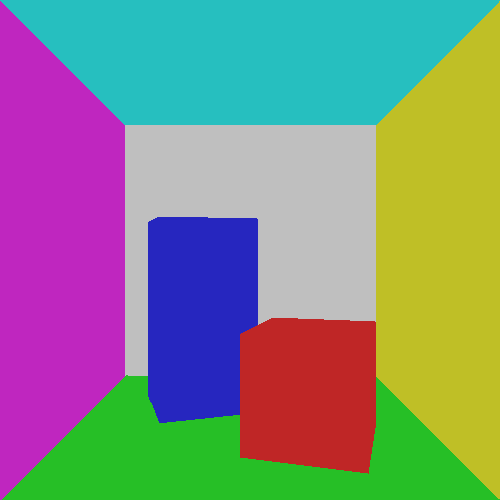
\includegraphics[width=0.45\linewidth]{screenshot2.png}
	\caption{The output when using a Z-Buffer}
	\label{fig2}
\end{figure}

\subsection{Lighting}
We implemented two ways to determine the direct lighting. The first one was calculating the direct light in each vertices and then interpolate the lighting for the rest of the polygon. This is shown below in figure \ref{fig3}. The second approach was to calculate the direct light for each pixel, see figure \ref{fig4} below. Nether of this approaches implements shadows on an object from an other object just the object itself. We also uses approximation of indirect light in the sam way as in lab 2.

\begin{figure}[h!]
	\centering
	\begin{subfigure}[h]{0.3\linewidth}
		\centering
		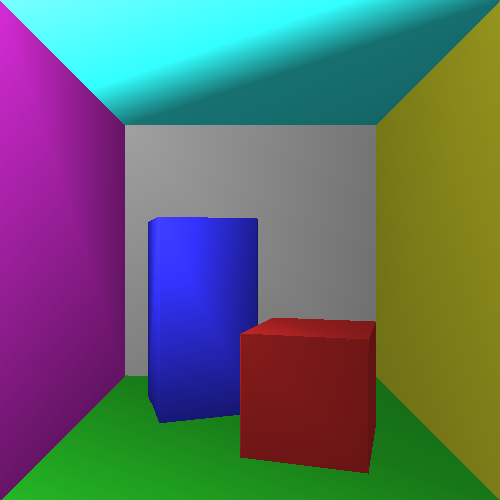
\includegraphics[width=\linewidth]{screenshot3.png}
		\caption{Light calculated per vertex}
		\label{fig3}
	\end{subfigure}
	\begin{subfigure}[h!]{0.3\linewidth}
		\centering
		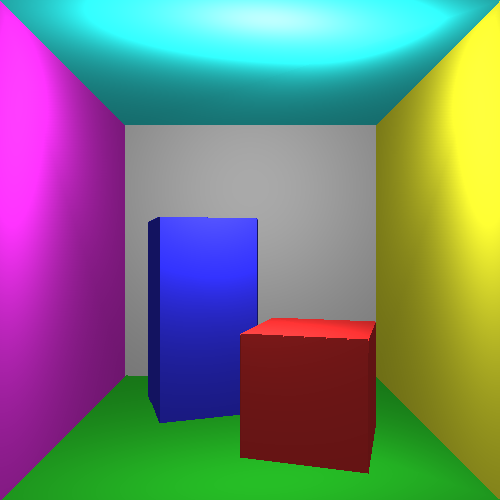
\includegraphics[width=\linewidth]{screenshot4.png}
		\caption{Light calculated per pixel}
		\label{fig4}
	\end{subfigure}
	\caption{Two different ways to calculate direct light}
\end{figure} 

As can be seen in the figures above the vertex version gets some anomalies when two polygons lies parallel to each other side by side, eg. the roof of the room. There is an anomaly in the pixel version to, if you look closely you can see that the shape of the light is a bit odd. This is caused by an incorrect interpolation, to fix this we had to do perspective correct interpolation instead of linear interpolation when calculating the direct light. We had some trouble doing this and the result of an incorrect implementation turd out to be pretty spectacular. (see figure \ref{fun} below)
\begin{figure}[h!]
	\centering
	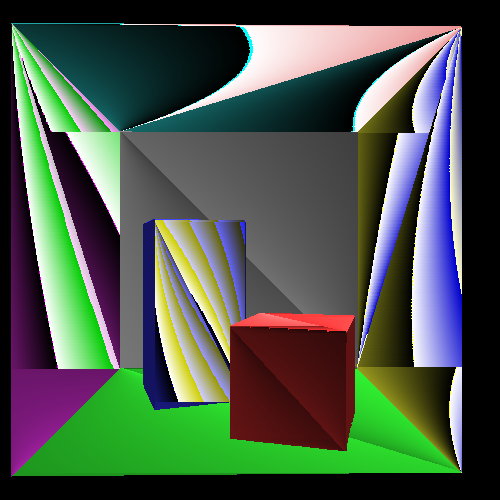
\includegraphics[width=0.45\linewidth]{fun.png}
	\caption{An incorrect implementation of perspective correct interpolation}
	\label{fun}
\end{figure}

\section{Result}
We had a lot more problem with this lab then the first two, but we are pleased with the result 


\section{just for fun}
 we did a fast implementation of the raytracing shadows in our rastarizer. Turned out that it was not that easy as just copying the functions needed and the point of using a rastarizer got lost due to the time consuming task to calculate shadows the raytracer way. Then we ran out of time do do it the proper way eg. with a shadow map.
\begin{figure}[h!]
	\centering
	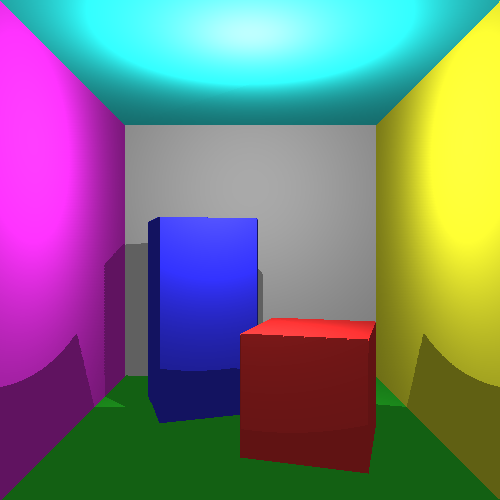
\includegraphics[width=0.45\linewidth]{shadows.png}
	\caption{An incorrect implementation of shadows}
	\label{shadows}
\end{figure}


\end{document}
